\documentclass[a3paper,12pt]{extarticle} % Use extarticle for A3 paper size
\usepackage{graphicx} % Include this package for \includegraphics
\usepackage{amsmath}
\usepackage{amssymb} % Include this package for \mathbb
\usepackage[margin=1in]{geometry} % Adjust the margin as needed
\usepackage{hyperref} % Include this package for \url

\begin{document}

\author{kipngeno koech - bkoech}
\title{Homework 1 - Introduction to Probabilistic Graphical Models}   
\maketitle

\medskip

\maketitle

\section{Bayesian Networks}

\begin{enumerate}
\item Consider a simple Markov Chain structure \( X \rightarrow Y \rightarrow Z \), where all variables are binary. You are required to:
\begin{enumerate}
    \item Write a code (using your preferred programming language) that generates a distribution (not necessarily a valid BN one) over the 3 variables.
        \[\textbf{[ in the notebook]}\]
    \item Write a code that verifies whether a distribution is a valid BN distribution.
        \[\textbf{[ in the notebook ]}\]
    \item Using your code, generate 10000 distributions and compute the fraction of distributions that are valid BN distributions.
        \[\textbf{ [ in the notebook ]}\]
\end{enumerate}
\item Given the following Bayesian Network
\begin{figure}[h]
    \centering
    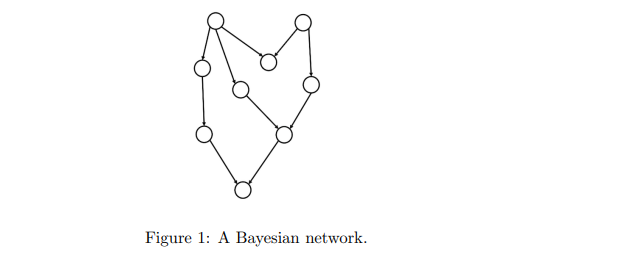
\includegraphics[width=0.5\textwidth]{bn.png}
    \caption{Bayesian Network}
\end{figure}
\begin{enumerate}
    \item Propose a topological ordering of this graph
    \begin{figure}[h]
        \centering
        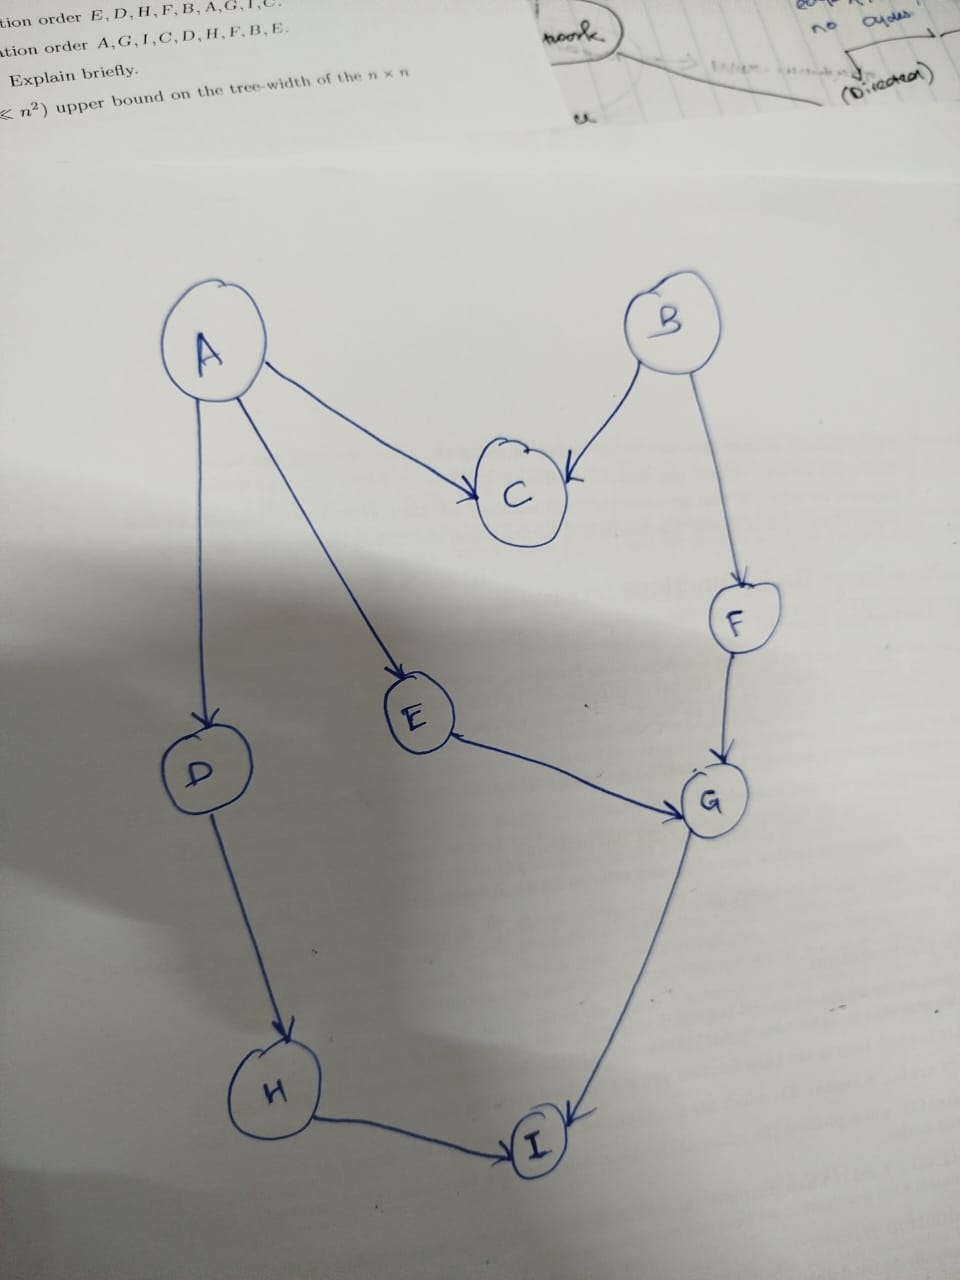
\includegraphics[width=0.5\textwidth]{bn1.jpg}
        \caption{Bayesian Network}
    \end{figure}
    \\ In Figure 2, the topological ordering is:
    \begin{enumerate}
        \item \(A \rightarrow B \rightarrow C \rightarrow D \rightarrow E \rightarrow F \rightarrow G \rightarrow H \rightarrow I \)
        \item \(A \rightarrow B \rightarrow C \rightarrow E \rightarrow D \rightarrow F \rightarrow G \rightarrow I \rightarrow H \)
    \end{enumerate}
    \item Let \(\textbf{X}\) be a random vector that is Markov with respect to the graph. We assume that the random variables X, are binary. Write all the local conditional independence
    \[
        X_A \text{ has no parents, so no independence condition applies here.} 
    \]
    \[
        X_B \text{ has no parents, so no independence condition applies here.} \\
    \]
    \(X_C \text{ is conditionally independent of all other nodes given its parent } X_A: \)
    \[
        X_C \perp \{X_B, X_D, X_E, X_F, X_G, X_H, X_I\} \mid X_A \\
    \]
    \(
        X_D \text{ is conditionally independent of all other nodes given its parent } X_A: \\
    \)
    \[
        X_D \perp \{X_B, X_C, X_E, X_F, X_G, X_H, X_I\} \mid X_A \\
    \]
    \(
        X_E \text{ is conditionally independent of all other nodes given its parents } X_C \text{ and } X_D: \\
    \)
    \[
        X_E \perp \{X_A, X_B, X_F, X_G, X_H, X_I\} \mid \{X_C, X_D\} \\
    \]
    \(
        X_F \text{ is conditionally independent of all other nodes given its parent } X_B: \\
    \)
    \[
        X_F \perp \{X_A, X_C, X_D, X_E, X_G, X_H, X_I\} \mid X_B \\
    \]
    \(
        X_G \text{ is conditionally independent of all other nodes given its parents } X_E \text{ and } X_F: \\
    \)
    \[
        X_G \perp \{X_A, X_B, X_C, X_D, X_H, X_I\} \mid \{X_E, X_F\} \\
    \]
    \(
        X_H \text{ is conditionally independent of all other nodes given its parent } X_D: \\
    \)
    \[
        X_H \perp \{X_A, X_B, X_C, X_E, X_F, X_G, X_I\} \mid X_D \\
    \]
    \(
        X_I \text{ is conditionally independent of all other nodes given its parents } X_G \text{ and } X_H: \\
    \)
    \[
        X_I \perp \{X_A, X_B, X_C, X_D, X_E, X_F\} \mid \{X_G, X_H\}
    \]
\end{enumerate}
\item  State True or False, and briefly justify your answer within 3 lines. The statements are either
direct consequences of theorems in Koller and Friedman (2009, Ch. 3), or have a short proof. In the
follows, P is a distribution and G is a BN structure.
\begin{enumerate}
    \item If \( A \perp B \mid C \) and \( A \perp C \mid B \), then \( A \perp B \) and \( A \perp C \). (Suppose the joint distribution of \( A, B, C \) is positive.) (This is a general probability question not related to BNs.)
    \begin{itemize}
        \item \textbf{False}. Whilst local independence implies global independence, global independence does not imply local independence.
    \end{itemize}
    \begin{figure}[h]
        \centering
        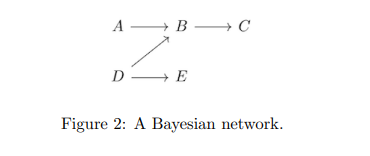
\includegraphics[width=0.5\textwidth]{bn2.png}
        \caption{Bayesian Network}
    \end{figure}
    \item In Figure 2, \(E \perp C \mid B\)
    \\ \textbf{True}. \(E\) is conditionally independent of \(C\) given \(B\) because we have conditioned on the node \(B\).
    \item in Figure 2, \(A \perp E \mid C\)
    \\ \textbf{False}. \(A\) is not conditionally independent of \(E\) given \(C\) because there is a path from \(A\) to \(E\) that is not blocked by \(C\).
    \begin{figure}[h]
        \centering
        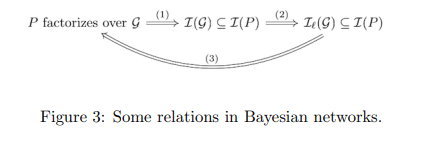
\includegraphics[width=0.5\textwidth]{bn3.png}
    \end{figure}
    \\\\ In figure 3, 
Recall the definitions of local and global independences of \( G \) and independences of \( P \).
\[
I_l(G) = \{(X \perp \text{NonDescendants}_G(X) \mid \text{Parents}_G(X))\} \tag{1}
\]
\[
I(G) = \{(X \perp Y \mid Z) : \text{d-separated}_G(X, Y \mid Z)\} \tag{2}
\]
\[
I(P) = \{(X \perp Y \mid Z) : P(X, Y \mid Z) = P(X \mid Z)P(Y \mid Z)\} \tag{3}
\]
\item In Figure 3, relation 1 is true.
\item In Figure 3, relation 2 is true.
\item In Figure 3, relation 3 is true.
\item If \( G \) is an I-map for \( P \), then \( P \) may have extra conditional independencies than \( G \).
\item Two BN structures \( G_1 \) and \( G_2 \) are I-equivalent if they have the same skeleton and the same set of v-structures.
\item If \( G_1 \) is an I-map of distribution \( P \), and \( G_1 \) has fewer edges than \( G_2 \), then \( G_2 \) is not a minimal I-map of \( P \).
\item The P-map of a distribution, if it exists, is unique.
\end{enumerate}
\end{enumerate}
\newpage
\section{Markov Networks}
Let \( \mathbf{X} = (X_1, \ldots, X_d) \) be a random vector with mean \( \boldsymbol{\mu} \) and covariance matrix \( \boldsymbol{\Sigma} \). The partial correlation matrix \( \mathbf{R} \) of \( \mathbf{X} \) is a \( d \times d \) matrix where each entry \( R_{ij} = \rho(X_i, X_j \mid \mathbf{X}_{-ij}) \) is the partial correlation between \( X_i \) and \( X_j \) given the \( d-2 \) remaining variables \( \mathbf{X}_{-ij} \). Let \( \boldsymbol{\Theta} = \boldsymbol{\Sigma}^{-1} \) be the inverse covariance matrix of \( \mathbf{X} \).

We will prove the relation between \( \mathbf{R} \) and \( \boldsymbol{\Theta} \), and furthermore how \( \boldsymbol{\Theta} \) characterizes conditional independence in Gaussian graphical models.

\begin{enumerate}
    \item (10 points) Show that
    \[
    \begin{pmatrix}
    \Theta_{ii} & \Theta_{ij} \\
    \Theta_{ji} & \Theta_{jj}
    \end{pmatrix}
    =
    \begin{pmatrix}
    \text{Var}[e_i] & \text{Cov}[e_i, e_j] \\
    \text{Cov}[e_i, e_j] & \text{Var}[e_j]
    \end{pmatrix}^{-1}
    \]
    for any \(i, j \in [d], i \neq j\). Here \(e_i\) is the residual resulting from the linear regression of \(X_{-ij}\) to \(X_i\), and similarly \(e_j\) is the residual resulting from the linear regression of \(X_{-ij}\) to \(X_j\).
    \\ The residuals \( e_i \) and \( e_j \) are given by:
   \[
   e_i = X_i - \mathbb{E}[X_i | X_{-ij}], \quad e_j = X_j - \mathbb{E}[X_j | X_{-ij}].
   \]
   These residuals are uncorrelated with \( X_{-ij} \), meaning \( \text{Cov}(e_i, X_{-ij}) = 0 \) and \( \text{Cov}(e_j, X_{-ij}) = 0 \).

\textbf{Covariance of Residuals:}
   The covariance matrix of the residuals \( e_i \) and \( e_j \) is:
   \[
   \text{Cov}(e_i, e_j) = \text{Cov}(X_i, X_j | X_{-ij}).
   \]
   This is because the residuals capture the conditional covariance between \( X_i \) and \( X_j \) given \( X_{-ij} \).

\textbf{Inverse Covariance Matrix:}
   The inverse covariance matrix \( \Theta = \Sigma^{-1} \) satisfies:
   \[
   \Theta = \begin{pmatrix}
   \Theta_{ii} & \Theta_{ij} \\
   \Theta_{ji} & \Theta_{jj}
   \end{pmatrix}.
   \]
   By the properties of the inverse covariance matrix, the conditional covariance matrix of \( (X_i, X_j) \) given \( X_{-ij} \) is:
   \[
   \text{Cov}(X_i, X_j | X_{-ij}) = \begin{pmatrix}
   \Theta_{ii} & \Theta_{ij} \\
   \Theta_{ji} & \Theta_{jj}
   \end{pmatrix}^{-1}.
   \]

\textbf{Equating the Matrices:}
   Since \( \text{Cov}(e_i, e_j) = \text{Cov}(X_i, X_j | X_{-ij}) \), we have:
   \[
   \begin{pmatrix}
   \Theta_{ii} & \Theta_{ij} \\
   \Theta_{ji} & \Theta_{jj}
   \end{pmatrix}
   =
   \begin{pmatrix}
   \text{Var}[e_i] & \text{Cov}[e_i, e_j] \\
   \text{Cov}[e_i, e_j] & \text{Var}[e_j]
   \end{pmatrix}^{-1}.
   \]
    \item (10 points) Show that
    \[
    R_{ij} = -\frac{\Theta_{ij}}{\sqrt{\Theta_{ii} \Theta_{jj}}}
    \]
    
\textbf{Partial Correlation:}
The partial correlation \( R_{ij} \) is defined as:
\[
R_{ij} = \rho(X_i, X_j | X_{-ij}) = \frac{\text{Cov}(X_i, X_j | X_{-ij})}{\sqrt{\text{Var}(X_i | X_{-ij}) \text{Var}(X_j | X_{-ij})}}.
\]

\textbf{Conditional Covariance and Variance:}
From Problem 1, we know:
\[
\text{Cov}(X_i, X_j | X_{-ij}) = -\frac{\Theta_{ij}}{\Theta_{ii} \Theta_{jj} - \Theta_{ij}^2},
\]
and:
\[
\text{Var}(X_i | X_{-ij}) = \frac{1}{\Theta_{ii}}, \quad \text{Var}(X_j | X_{-ij}) = \frac{1}{\Theta_{jj}}.
\]

\textbf{Substitute into Partial Correlation:}
Substituting these into the definition of \( R_{ij} \), we get:
\[
R_{ij} = \frac{-\frac{\Theta_{ij}}{\Theta_{ii} \Theta_{jj} - \Theta_{ij}^2}}{\sqrt{\frac{1}{\Theta_{ii}} \cdot \frac{1}{\Theta_{jj}}}}.
\]
Simplifying, we obtain:
\[
R_{ij} = -\frac{\Theta_{ij}}{\sqrt{\Theta_{ii} \Theta_{jj}}}.
\]

    
    \item (15 points) From the above result and the relation between independence and correlation, we know
    \[
    \Theta_{ij} = 0 \iff R_{ij} = 0 \implies X_i \perp X_j \mid X_{-ij}
    \]
    Note the last implication only holds in one direction. Now suppose \(X \sim N(\mu, \Sigma)\) is jointly Gaussian. Show that \(R_{ij} = 0 \implies X_i \perp X_j \mid X_{-ij}\).

    \textbf{Partial Correlation and Conditional Independence:}
From Problem 2, we know:
\[
R_{ij} = -\frac{\Theta_{ij}}{\sqrt{\Theta_{ii} \Theta_{jj}}}.
\]
If \( R_{ij} = 0 \), then \( \Theta_{ij} = 0 \).

\textbf{Inverse Covariance and Conditional Independence:}
For a jointly Gaussian distribution, the inverse covariance matrix \( \Theta = \Sigma^{-1} \) encodes conditional independence. Specifically:
\[
\Theta_{ij} = 0 \iff X_i \perp X_j | X_{-ij}.
\]
This is because the off-diagonal elements of \( \Theta \) represent the conditional dependence between variables after accounting for all other variables.

\textbf{Conclusion:}
Since \( R_{ij} = 0 \) implies \( \Theta_{ij} = 0 \), it follows that:
\[
X_i \perp X_j | X_{-ij}.
\]

\end{enumerate}
\newpage

\section{Exact Inference - Variable Elimination}

Reference materials for this problem:
\begin{itemize}
    \item Jordan textbook Ch. 3, available at \url{https://people.eecs.berkeley.edu/~jordan/prelims/chapter3.pdf}
    \item Koller and Friedman (2009, Ch. 9 and Ch. 10)
\end{itemize}

\subsection{Variable elimination on a grid [10 points]}
Consider the following Markov network:
\begin{figure}[h]
    \centering
    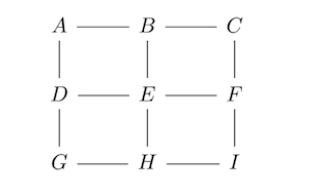
\includegraphics[width=0.5\textwidth]{bn4.png}
    \caption{Markov Network}
\end{figure}

We are going to see how tree-width, a property of the graph, is related to the intrinsic complexity of
variable elimination of a distribution

\begin{enumerate}
\item (5 points) Write down largest clique(s) for the elimination order \(E, D, H, F, B, A, G, I, C\).
\\ We start by eliminating \(E\), its neighbors are \(D, F, H, B\), so the clique here is :\(\{D, F, H, B\}\). size: \(\textbf{4}\)
\\ We then eliminate \(D\), its neighbors are \(A, B, F, G, H\), so the clique here is: \(\{A, B, f, G, H\}\). size: \(\textbf{5}\)
\\ We then eliminate \(H\), its neighbors are \(G, A, I, B, F\), so the clique here is: \(\{G, A, I, B, F\}\). size: \(\textbf{5}\)
\\ We then eliminate \(F\), its neighbors are \(A, B, c, G, I\), so the clique here is: \(\{A, B, C, G, I\}\). size: \(\textbf{5}\)
\\ We then eliminate \(B\), its neighbors are \(A, C, G, I\), so the clique here is: \(\{A, C, G, I\}\). size: \(\textbf{4}\)
\\ We then eliminate \(A\), its neighbors are \(C, G, I\), so the clique here is: \(\{C, G, I\}\). size: \(\textbf{3}\)
\\ We then eliminate \(G\), its neighbors are \(C, I\), so the clique here is: \(\{C, I\}\). size: \(\textbf{2}\)
\\ We then eliminate \(I\), its neighbors are \(C\), so the clique here is: \(\{C\}\). size: \(\textbf{1}\)
\\ The largest clique(s) for the elimination order \(E, D, H, F, B, A, G, I, C\) is \textbf{5}

\item (5 points) Write down largest clique(s) for the elimination order \(A, G, I, C, D, H, F, B, E\).
\\ We start by eliminating \(A\), its neighbors are \(D, B\), so the clique here is: \(\{D, B\}\). size: \(\textbf{2}\)
\\ We then eliminate \(G\), its neighbors are \(D, H\),     so the clique here is: \(\{D, H\}\). size: \(\textbf{2}\)
\\ We then eliminate \(I\), its neighbors are \(H, F\), so the clique here is: \(\{H, F\}\). size: \(\textbf{2}\)
\\ We then eliminate \(C\), its neighbors are \(F, B\), so the clique here is: \(\{F, B\}\). size: \(\textbf{2}\)
\\ We then eliminate \(D\), its neighbors are \(H, B, E\), so the clique here is: \(\{H, B, E\}\). size: \(\textbf{3}\)
\\ We then eliminate \(H\), its neighbors are \(F, B, E\), so the clique here is: \(\{F, B, E\}\). size: \(\textbf{3}\)
\\ We then eliminate \(F\), its neighbors are \(B, E\), so the clique here is: \(\{B, E\}\). size: \(\textbf{2}\)
\\ We then eliminate \(B\), its neighbors are \(E\), so the clique here is: \(\{E\}\). size: \(\textbf{1}\)
\\ The largest clique(s) for the elimination order \(A, G, I, C, D, H, F, B, E\) is \textbf{3}

\item (5 points) Which of the above ordering is preferable? Explain briefly.
\\ The second ordering is preferable because it results in a smaller largest clique size (3) compared to the first ordering (5). A smaller clique size generally leads to more efficient computations in variable elimination algorithms.

\item (10 points) Using this intuition, give a reasonable (\(\ll n^2\)) upper bound on the tree-width of the \(n \times n\) grid.
\\ The tree-width of an \(n \times n\) grid is at most \(2n - 2\). This is because the grid can be decomposed into a tree structure where each node has at most \(2n - 2\) neighbors. This upper bound is reasonable and much smaller than \(n^2\), which would be the case for a fully connected graph.
\end{enumerate}

\end{document}